\documentclass{article}
\usepackage{tikz}
\usetikzlibrary{shapes.geometric}

\begin{document}

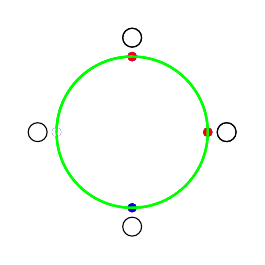
\begin{tikzpicture}[scale=1.2]
    % Define the number of nodes
    \def\nodes{5}
    
    % Loop through each node to draw the diagrams
    \foreach \i in {0,...,\nodes} {
        \pgfmathtruncatemacro{\j}{mod(\i+1, \nodes)}
        \pgfmathtruncatemacro{\k}{mod(\i+2, \nodes)}
        
        % Draw the circle
        \draw (90*\i:1) circle (0.1);
        
        % Draw the nodes
        \fill[blue] (90*\i:0.8) circle (0.05) node[above] {};
        \fill[red] (90*\j:0.8) circle (0.05) node[above] {};
        \fill[white] (90*\k:0.8) circle (0.05) node[above] {};
        
        % Draw the green link
        \draw[green, thick] (90*\i:0.8) arc (90*\i:90*\j:0.8);
    }
    
    % Draw the green link for the last diagram
    \draw[green, thick] (90*\nodes:0.8) arc (90*\nodes:90*(\nodes+1):0.8);
\end{tikzpicture}

\end{document}